\documentclass[10pt,hyperref={colorlinks,citecolor=blue,urlcolor=peking_blue,linkcolor=}]{beamer}
\usepackage{bydevmar}
\usefonttheme{serif}
\usepackage{lipsum}
%\usepackage[scheme = plain]{ctex}
\usepackage{hyperref}
\usepackage{charter} % Nicer fonts
% other packages
\usepackage{latexsym,amsmath,xcolor,multicol,booktabs,calligra}
\usepackage{amssymb}
\usepackage{graphicx}
\usepackage{bm}
\usepackage{natbib}
\usepackage{wrapfig}
\usepackage{amsfonts} 
\usepackage{ragged2e}
\usepackage{parskip}

\usepackage{caption}

\apptocmd{\frame}{}{\justifying}{} % Allow optional arguments after frame.

\newcommand{\theHalgorithm}{\arabic{algorithm}}
\theoremstyle{plain}
\newtheorem{axiom}{Axiom}
\newtheorem{claim}[axiom]{Claim}
\newtheorem{assumption}{Assumption}
\newtheorem{remark}{Remark}
\newtheorem{proposition}{Proposition}
\setbeamertemplate{theorems}[numbered] 


% change for your title page information
\author[BOUHLALI Abdelfattah]{BOUHLALI Abdelfattah}
\title{Analyse des sentiments avec NLP}
\subtitle{}
\institute{Master Mathématiques Appliquées pour la Science des Données}
\date{2023 - 2024}


\newif\ifplacelogo % create a new conditional
\placelogotrue % set it to true
\logo{
\ifplacelogo

\includegraphics[width=2cm]{Figures/fpo_logo.png}
\fi
  
}
% official colors match with the PKU red
\def\cmd#1{\texttt{\color{red}\footnotesize $\backslash$#1}}
\def\env#1{\texttt{\color{blue}\footnotesize #1}}
\definecolor{deepblue}{rgb}{0,0,0.5}
\definecolor{deepred}{rgb}{0.6,0,0}
\definecolor{deepgreen}{rgb}{0,0.5,0}
\definecolor{halfgray}{gray}{0.55}

\begin{document}
{
\setbeamertemplate{logo}{}
\begin{frame}
    \titlepage
    \begin{figure}[htpb]
        \begin{center}
        
            
\includegraphics[width=0.2\linewidth]{Figures/imogies.jpg}\\
            
            
\includegraphics[width=0.3\linewidth]{Figures/fpo_logo.png} \\
            
            \emph{\textbf{Encadré par :}}\\ 
            \textsc{GAOU Salma} \\
            \textsc{HAMIDI Charaf}
            
        \end{center}
    \end{figure}
\end{frame}
}

\placelogofalse
% -Introduction
\section{Introduction}

\begin{frame}
    \frametitle{Introduction}

    \begin{itemize}
        \item Notre projet explore les avis des consommateurs sur Amazon, en se concentrant sur les produits alimentaires.
        \item Le défi est de comprendre ce que les clients pensent vraiment. Avec tant d'avis, il est difficile de trouver les informations importantes.
        \item Nous voulons transformer ces avis en idées utiles pour aider les entreprises à améliorer leurs produits et à satisfaire les clients.
    \end{itemize}
\end{frame}

\subsection{Problème ou Question à Résoudre}

\begin{frame}
    \frametitle{Problème ou Question à Résoudre}

    \begin{itemize}
        \item On essaie de comprendre les avis des gens sur les produits alimentaires d'Amazon.
        \item Comment les clients se sentent-ils vraiment? C'est difficile car il y a beaucoup d'avis.
        \item Notre but est de trouver des informations importantes pour aider les entreprises.
    \end{itemize}
\end{frame}

\subsection{Contexte et Motivation}

\begin{frame}
    \frametitle{Contexte et Motivation}

    \begin{itemize}
        \item Beaucoup de gens achètent sur Amazon, et ils laissent beaucoup d'avis.
        \item Mais ces avis ne sont pas toujours faciles à comprendre. Nous voulons aider les entreprises à comprendre ce que les clients aiment et n'aiment pas.
    \end{itemize}
\end{frame}

\subsection{Objectifs du Projet et Hypothèses à Tester}

\begin{frame}
    \frametitle{Objectifs du Projet et Hypothèses à Tester}

    \textbf{Objectifs du Projet :}

    \begin{enumerate}
        \item Comprendre les Sentiments.
        \item Identifier les Tendances.
        \item Améliorer la Pertinence.
    \end{enumerate}

    \textbf{Hypothèses à Tester :}

    \begin{enumerate}
        \item Les sentiments des clients varient en fonction des types de produits alimentaires.
        \item Certains mots-clés auront une influence significative sur la perception des produits.
        \item Les tendances dans les avis sur les produits alimentaires évoluent avec le temps.
    \end{enumerate}
\end{frame}

% -Methodologie
\section{Méthodologie}

\begin{frame}{Definition, Proposition and Theorem}

\begin{definition}[some explanations]
\lipsum[3][1-4]
\end{definition}

\begin{proposition}\label{prop:1}
\lipsum[3][5-8]
\end{proposition}

\begin{theorem}\label{theorem:generalization bound}
\lipsum[3][9-12]
\end{theorem}
    
\end{frame}


% - Resultats
\section{Resultats}

% - Discussion
\section{Discussion}

\begin{frame}
    \frametitle{Points forts de RoBERTa}
    \begin{itemize}
        \item Compréhension fine des sentiments : RoBERTa excelle dans la compréhension fine des sentiments exprimés dans les avis, en distinguant clairement entre les sentiments positifs, négatifs et neutres.

        \item Capacité à identifier les tendances : RoBERTa peut découvrir les tendances émergentes dans les avis, y compris les préférences alimentaires, les aspects appréciés ou critiqués, offrant ainsi des informations précieuses sur les évolutions du marché.

        \item Analyse de mots clés et d'expressions fréquemment utilisés : RoBERTa peut aider à déterminer les aspects importants en analysant les mots clés et les expressions fréquemment utilisés dans les avis, permettant une identification rapide des points forts ou des points faibles des produits.
    \end{itemize}
\end{frame}


\begin{frame}
    \frametitle{Limites de RoBERTa}
    \begin{itemize}
        \item Dépendance aux données d'entraînement : RoBERTa dépend fortement des données sur lesquelles il a été formé, ce qui peut affecter sa précision.
        \item Interprétation des résultats : Les modèles NLP complexes comme RoBERTa peuvent être difficiles à interpréter, rendant délicate l'interprétation des résultats.
        \item Besoin de ressources informatiques importantes : RoBERTa nécessite des ressources informatiques importantes pour son utilisation.
    \end{itemize}
\end{frame}
\begin{frame}
    \frametitle{Limites de RoBERTa}
    \begin{itemize}
    
        \item Des Textes mal Classés : Malgré la plupart des classifications correctes, il peut y avoir des textes mal classés en raison de nuances linguistiques.
        
        \begin{figure}[h]
            \centering
            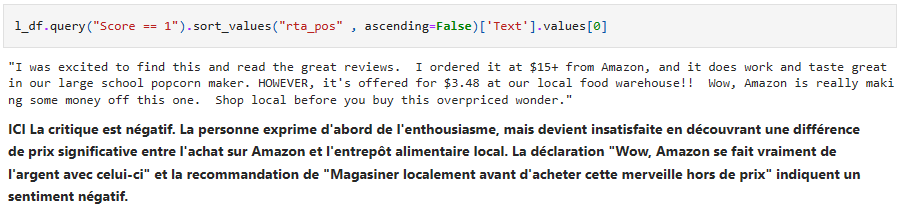
\includegraphics[scale=0.4]{Figures/pointsfaible1.png}
            \caption{Limites de RoBERTa : Example 1 }
            \label{fig:Limit1RoBERTa}
        \end{figure}

        \begin{figure}[h]
            \centering
            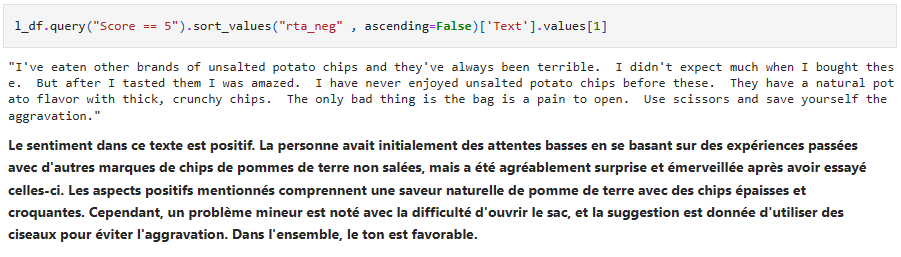
\includegraphics[scale=0.3]{Figures/pointsfaible2.png}
            \caption{Limites de RoBERTa : Example 2 }
            \label{fig:Limit2RoBERTa}
        \end{figure}
        
    \end{itemize}
\end{frame}

\begin{frame}
    \frametitle{Suggestions et améliorations possibles du projet}
    \begin{itemize}
        \item Exploration de sous-catégories alimentaires : Explorer les sentiments dans des sous-catégories spécifiques de produits alimentaires pour obtenir des informations plus détaillées.
        \item Enrichissement du modèle avec des données spécifiques au domaine : Utiliser des données spécifiques au domaine alimentaire pour enrichir le modèle.
        \item Intégration de la rétroaction des entreprises : Permettre aux entreprises de répondre aux avis pourrait offrir une perspective plus complète sur la satisfaction du client.
        \item Analyse de la dynamique temporelle : Investiguer les tendances au fil du temps en analysant les changements mensuels dans les avis.
        \item Comparaison avec d'autres modèles NLP : Comparer avec d'autres modèles NLP pour évaluer la performance relative.
    \end{itemize}
\end{frame}

\begin{frame}
    \frametitle{Implications et conclusions tirées des résultats obtenus}
    \begin{itemize}
        \item Tendance positive globale : La distribution des scores suggère une tendance positive globale dans les avis des clients sur les produits alimentaires d'Amazon.
        \item Importance des avis avec des scores élevés : La majorité des scores sont entre 4 et 5, soulignant l'importance des avis positifs.
        \item Prévalence des évaluations positives : La fréquence élevée des évaluations positives, en particulier avec un score de 5, peut indiquer une propension des utilisateurs à partager leurs expériences positives.
    \end{itemize}
\end{frame}


% - Conclusion



\section{Conclusion}
% Recap
\subsection{Récapitulation des Principaux Résultats:}

1. Tendance Globale Positive: L'analyse des scores des avis suggère une tendance globale positive, avec une prédominance d'évaluations élevées, principalement de 4 et 5.

2. Identification de Tendances Alimentaires: RoBERTa a été utilisé avec succès pour identifier des tendances émergentes dans les avis, notamment des préférences alimentaires, des aspects appréciés ou critiqués spécifiques, et des évolutions au fil du temps.

3. Importance des Avis Positifs: Les avis positifs avec des scores élevés sont prédominants, indiquant que la satisfaction des clients est généralement élevée.




% Repondre a la Question Initiale


\subsection{Réponse à la Question Initiale:}

La question initiale visait à comprendre les avis des clients sur les produits alimentaires d'Amazon. Les résultats obtenus suggèrent que la majorité des clients expriment des sentiments positifs envers ces produits. La satisfaction semble être élevée, ce qui peut être une information précieuse pour les entreprises cherchant à améliorer leurs produits.

\subsection{Contributions du Projet à la Connaissance du Domaine:}

1. Analyse Fine des Sentiments:L'utilisation de RoBERTa a permis une analyse fine des sentiments exprimés dans les avis, offrant une compréhension approfondie des opinions des clients.

2. Identification de Tendances et de Préférences: Le projet a contribué à l'identification de tendances émergentes et de préférences alimentaires, offrant ainsi des informations utiles pour les entreprises cherchant à répondre aux attentes du marché.

3. Utilisation de Données Réelles d'Amazon: En utilisant un ensemble de données provenant des avis réels des clients sur Amazon, le projet a contribué à une analyse basée sur des données concrètes, renforçant ainsi la validité des résultats.

En conclusion, ce projet a fourni des informations précieuses sur les sentiments des clients à l'égard des produits alimentaires d'Amazon, mettant en lumière des tendances, des préférences et des points forts. Ces connaissances peuvent être exploitées par les entreprises pour améliorer leurs produits et satisfaire davantage leurs clients.


% - References

\section{Références}
\begin{frame}{Frame Title}
    \begin{thebibliography}{15}

\bibitem{xinyue2022amazon}
Xinyue Zhao et Yuandong Sun. (2022). "Amazon Fine Food Reviews with BERT Model." Procedia Computer Science, Volume 208, Pages 401-406. DOI: 10.1016/j.procs.2022.10.056. Elsevier B.V. Available online at: \url{https://www.sciencedirect.com/science/article/pii/S1877050922030215}.

\bibitem{huggingface2022roberta}
Hugging Face. (2022). Documentation Transformers - Modèle RoBERTa. \url{https://huggingface.co/docs/transformers/model_doc/roberta}.

\bibitem{mulla2022sentiment}
Mulla, R. (2022). Projet d'analyse de sentiment en Python avec NLTK et  Transformers. Classifiez les critiques d'Amazon !! [Vidéo]. YouTube. \url{https://www.youtube.com/watch?v=QpzMWQvxXWk}.

\bibitem{robikscube2022sentiment}
Robikscube. (2022). Analyse de sentiment en Python  [Didacticiel sur YouTube]. Kaggle. \url{https://www.kaggle.com/code/robikscube/sentiment-analysis-python-youtube-tutorial/notebook}.

% Ajoutez ici d'autres références au besoin...

\end{thebibliography}
\end{frame}

\end{document}